\documentclass[12pt]{article}

% --- SSRN-style working paper: single column, Times, 1.5 spacing ---
\usepackage[utf8]{inputenc}
\usepackage[T1]{fontenc}
\usepackage{mathptmx}                 % Times text + math (base)
\usepackage[margin=1in]{geometry}
\usepackage{setspace}
\usepackage{amsmath,amssymb,amsthm,mathtools}
\usepackage{graphicx}
\usepackage{booktabs}
\usepackage{caption}
\usepackage{abstract}
\usepackage{natbib}
\usepackage[hidelinks]{hyperref}

\onehalfspacing
\setlength{\parindent}{1.5em}
\captionsetup{font=small,labelfont=bf}
\renewcommand{\abstractnamefont}{\normalfont\bfseries}
\renewcommand{\abstracttextfont}{\normalfont\small}

\newtheorem{theorem}{Theorem}
\newtheorem{proposition}{Proposition}
\newtheorem{lemma}{Lemma}
\newtheorem{definition}{Definition}

\newcommand{\E}{\mathbb{E}}
\newcommand{\Cov}{\operatorname{Cov}}
\newcommand{\PD}{\mathrm{PD}}
\newcommand{\EPE}{\mathrm{EPE}}
\newcommand{\ENE}{\mathrm{ENE}}
\newcommand{\PFE}{\mathrm{PFE}}
\newcommand{\EEPE}{\mathrm{EEPE}}
\newcommand{\EE}{\mathrm{EE}}
\newcommand{\CVA}{\mathrm{CVA}}
\newcommand{\EAD}{\mathrm{EAD}}

\begin{document}

\begin{center}
{\LARGE\bfseries wayfault: A Minimal Hexagonal Library for\\[2pt]
Wrong-Way Risk with Prescriptive Inverse Calibration\par}
\vspace{1.2em}
{\large Dairon Aldaz\par}
\vspace{0.4em}
{\normalsize Independent\par}
\vspace{0.3em}
{\normalsize This version: \today\par}
\end{center}

\vspace{0.6em}

\begin{abstract}
\noindent
Wrong-way risk (WWR) is the adverse dependence between a counterparty's
exposure and its credit quality: exposure tends to be large precisely when the
counterparty is likely to default. We present \emph{wayfault}, a small,
dependency-light (numpy-only core) open-source Python library that quantifies
WWR for a single counterparty from a Monte-Carlo exposure cube and a credit
curve. The library computes baseline exposure metrics and unilateral credit
valuation adjustment (CVA), a \emph{conditional expected exposure given default}
under a pluggable dependence model, the WWR-adjusted CVA, and the empirical
multiplier $\alpha=\CVA_{\text{WWR}}/\CVA_{\text{indep}}$. We unify the
Hull--White stochastic-hazard model and the Gaussian, Clayton, and Frank copulas
under a single \emph{scenario re-weighting} core. Our main contribution is a
\emph{prescriptive inverse calibration}: given the proven monotonicity of
$\alpha$ in the dependence parameter, we root-find the parameter that reproduces
a \emph{target} multiplier or CVA, and we locate reverse-stress
\emph{breakpoints} at which a risk metric crosses a threshold. All structural
identities used by the implementation are machine-checked symbolically with a
computer-algebra system, and we report a worked example on a five-year swap.
\end{abstract}

\vspace{0.4em}
\noindent\textbf{Keywords:} wrong-way risk; credit valuation adjustment (CVA);
counterparty credit risk; xVA; copula; Hull--White model; reverse stress
testing; calibration; open-source software.

\vspace{0.3em}
\noindent\textbf{JEL Classification:} G13; G32; G17; C63.

\vspace{1.0em}

\section{Introduction}
Counterparty credit risk pricing charges a credit valuation adjustment (CVA)
for the expected loss from a counterparty defaulting while owing a positive
mark-to-market. The standard CVA computation assumes \emph{independence} between
exposure and default. Wrong-way risk (WWR) is the violation of this assumption
in the adverse direction; its favourable mirror is right-way risk
(RWR)~\citep{hullwhite2012,gregory}. WWR can materially raise CVA and the
regulatory exposure-at-default, yet practical, auditable, and dependency-light
tooling is scarce.

\emph{wayfault} targets this gap with a strict \emph{hexagonal} (ports and
adapters) design: a pure domain (standard library and numpy only), surrounded by
protocol ports and swappable adapters for exposure sources, credit curves,
dependence models, calibrators, and result sinks. Beyond the descriptive
pipeline, we contribute an \emph{inverse} layer that turns the tool
prescriptive. Section~\ref{sec:model} fixes notation;
Sections~\ref{sec:dep}--\ref{sec:metrics} define the dependence models and WWR
metrics; Section~\ref{sec:inverse} presents the inverse calibration and its
convergence; Section~\ref{sec:num} reports numerics; and Section~\ref{sec:verif}
describes the symbolic verification.

\section{Exposure, credit, and baseline metrics}\label{sec:model}
Let $0<t_1<\dots<t_n$ be a tenor grid with increments
$\Delta t_i=t_i-t_{i-1}$ ($t_0:=0$). The \emph{exposure cube} is a matrix
$V\in\mathbb{R}^{S\times n}$ of netting-set values over $S$ Monte-Carlo
scenarios. Write $V_s(t_i)$ for entry $(s,i)$ and $x^{+}=\max(x,0)$.

\paragraph{Exposure metrics.} The expected positive and negative exposure and
the potential future exposure at quantile $q$ are
\begin{align}
\EPE(t_i) &= \E\!\big[V(t_i)^{+}\big],\quad
\ENE(t_i) = \E\!\big[(-V(t_i))^{+}\big],\\
\PFE_q(t_i) &= \inf\{x:\Pr(V(t_i)^{+}\le x)\ge q\},
\end{align}
estimated by the sample mean and empirical quantile over scenarios. The
effective EPE is the time-weighted running maximum
\begin{equation}
\EEPE = \frac{1}{t_n}\sum_{i=1}^{n}\Big(\max_{j\le i}\EPE(t_j)\Big)\,\Delta t_i .
\end{equation}

\paragraph{Credit curve.} The counterparty is described by a piecewise-constant
hazard $\lambda(t)\ge 0$ (a flat curve being the single-segment case), giving
the survival and marginal default probabilities
\begin{equation}
S(t)=\exp\!\Big(-\!\int_0^t\!\lambda(u)\,du\Big),\quad
\PD(t_{i-1},t_i)=S(t_{i-1})-S(t_i),
\end{equation}
with recovery $R\in[0,1)$ and loss-given-default $1-R$. The marginal PDs
telescope, $\sum_{i=1}^{n}\PD(t_{i-1},t_i)+S(t_n)=1$.

\paragraph{Baseline CVA.} With discount factors $DF(t_i)$ and discounted
expected exposure $\EE(t_i)$, the unilateral CVA is
\begin{equation}\label{eq:cva}
\CVA=(1-R)\sum_{i=1}^{n}DF(t_i)\,\EE(t_i)\,\PD(t_{i-1},t_i).
\end{equation}

\section{Dependence via scenario re-weighting}\label{sec:dep}
WWR is injected by replacing the unconditional exposure expectation at each
tenor with a \emph{conditional} one, computed by re-weighting scenarios toward
those in which the counterparty is more likely to default. For tenor $i$ with
non-negative weights $w_{s,i}$ summing to one over $s$,
\begin{equation}\label{eq:condee}
\EE^{\mathrm{cond}}(t_i)=\sum_{s=1}^{S} V_s(t_i)^{+}\,w_{s,i}.
\end{equation}
Each dependence model supplies the weights.

\paragraph{Hull--White hazard.} Following~\citet{hullwhite2012} the default
intensity is coupled to portfolio value,
$\lambda(t)=\exp\!\big(a(t)+b\,V(t)\big)$, where $a(t)$ is fixed per tenor to
match the marginal PDs and $b$ is the wrong-way knob. The re-weighting is the
numerically stabilised softmax
\begin{equation}\label{eq:hwweights}
w_{s,i}=\frac{e^{\,b\,V_s(t_i)}}{\sum_{k=1}^{S} e^{\,b\,V_k(t_i)}}.
\end{equation}

\paragraph{Gaussian copula.} With a one-factor latent
$X=\rho M+\sqrt{1-\rho^2}\,Z$ and default when $X\le\Phi^{-1}(p_i)$, conditioning
on the (rank-normalised) market score $y_s$ gives the per-scenario default
probability
\begin{equation}\label{eq:gauss}
w_{s,i}\propto
\Phi\!\left(\frac{\Phi^{-1}(p_i)+\rho\,y_s}{\sqrt{1-\rho^2}}\right),
\end{equation}
where $p_i=\PD(t_{i-1},t_i)$ and $\Phi$ is the standard normal CDF.

\paragraph{Archimedean copulas.} For an Archimedean copula $C(u,v)$ the
conditional default ``grade'' is the $h$-function $h(u\mid v)=\partial_v C(u,v)$,
evaluated at $u=p_i$ and the market grade $v_s$. The Clayton and Frank
generators yield the closed forms
\begin{align}
h_{\text{Cl}}(u\mid v)&=v^{-(\theta+1)}\big(u^{-\theta}+v^{-\theta}-1\big)^{-\frac{\theta+1}{\theta}},
\label{eq:clayton}\\
h_{\text{Fr}}(u\mid v)&=\frac{e^{-\theta v}\,(e^{-\theta u}-1)}
{(e^{-\theta}-1)+(e^{-\theta u}-1)(e^{-\theta v}-1)}.
\label{eq:frank}
\end{align}
Clayton ($\theta>0$) carries lower-tail dependence (defaults cluster with high
exposure); Frank is symmetric and its sign selects the direction.

\section{Wrong-way risk metrics}\label{sec:metrics}
Re-evaluating~\eqref{eq:cva} with the conditional exposure~\eqref{eq:condee}
gives the WWR-adjusted $\CVA_{\text{WWR}}$. The empirical multiplier and the
exposure-at-default view are
\begin{equation}
\alpha=\frac{\CVA_{\text{WWR}}}{\CVA_{\text{indep}}},\qquad
\EAD=\alpha\cdot\EEPE .
\end{equation}
A counterparty is labelled \textsc{wrong-way} when the dependence parameter is
positive and $\alpha>1$, \textsc{right-way} when negative and $\alpha<1$, and
\textsc{neutral} otherwise.

\subsection{Arbitrage consistency}
A calibrated model must reproduce the curve's marginal PDs when integrated over
exposure, otherwise it mis-prices the unconditional default.

\begin{proposition}[Marginal consistency]\label{prop:marg}
Define the per-scenario interval default probability
$q_i(s)=p_i\,w_{s,i}\,S$ with the softmax weights~\eqref{eq:hwweights} and $S$
scenarios. Then its scenario mean equals the target,
$\tfrac{1}{S}\sum_s q_i(s)=p_i$.
\end{proposition}
\begin{proof}
Since $\sum_s w_{s,i}=1$,
$\tfrac1S\sum_s p_i\,w_{s,i}\,S=p_i\sum_s w_{s,i}=p_i.$
\end{proof}

\section{Monotonicity and inverse calibration}\label{sec:inverse}
The descriptive map $b\mapsto\alpha(b)$ admits a clean monotonicity, which is
the engine of the inverse layer.

\begin{lemma}[Score identity]\label{lem:cov}
For softmax weights $w_s(b)=e^{bV_s}/\sum_k e^{bV_k}$ and any
$f:\mathbb{R}\to\mathbb{R}$ with $f_s=f(V_s)$,
\begin{equation}
\frac{d}{db}\,\E_{w}[f]=\Cov_{w}(f,V),
\end{equation}
where $\E_w[\cdot]$ and $\Cov_w$ are taken under $w(b)$.
\end{lemma}
\begin{proof}
Differentiating $\E_w[f]=\sum_s f_s e^{bV_s}/\sum_k e^{bV_k}$ in $b$ gives
$\E_w[fV]-\E_w[f]\E_w[V]=\Cov_w(f,V)$.
\end{proof}

\begin{theorem}[Monotone WWR]\label{thm:mono}
At every tenor, $\EE^{\mathrm{cond}}(t_i)$ is nondecreasing in $b$. Consequently
$\CVA_{\text{WWR}}$ and $\alpha$ are nondecreasing in $b$, with $\alpha\ge1$ for
$b>0$ and $\alpha\le1$ for $b<0$; at $b=0$ the construction reduces to the
independent case and $\alpha=1$.
\end{theorem}
\begin{proof}
Apply Lemma~\ref{lem:cov} with $f(V)=V^{+}$. Because $V^{+}$ is nondecreasing in
$V$, $f$ and the identity are comonotone, so by the Chebyshev sum inequality
$\Cov_w(V^{+},V)\ge0$; hence $\partial_b\EE^{\mathrm{cond}}(t_i)\ge0$. As
$\EE\ge0$ and the PDs and discount factors in~\eqref{eq:cva} are non-negative,
$\CVA_{\text{WWR}}$ inherits monotonicity, and so does
$\alpha=\CVA_{\text{WWR}}/\CVA_{\text{indep}}$. At $b=0$ the weights are uniform
and~\eqref{eq:condee} is the sample mean, i.e.\ the baseline.
\end{proof}

\subsection{The inverse problem}
Let $g(\beta)$ denote a WWR metric (e.g.\ $\alpha$, $\CVA_{\text{WWR}}$, or
$\EAD$) as a function of a scalar dependence parameter $\beta$ supplied through a
model factory. By Theorem~\ref{thm:mono} (and its copula analogues) $g$ is
monotone, hence injective on any bracket
$[\beta_{\mathrm{lo}},\beta_{\mathrm{hi}}]$.

\begin{definition}[Target calibration and breakpoint]
Given a target $g^\star$ with
$g(\beta_{\mathrm{lo}})\le g^\star\le g(\beta_{\mathrm{hi}})$, the inverse
problem seeks $\beta^\star$ with $g(\beta^\star)=g^\star$. When $g^\star$ is a
risk \emph{threshold} (capital breach, internal limit) the solution is the
reverse-stress \emph{breakpoint}.
\end{definition}

\begin{proposition}[Existence, uniqueness, convergence]
If $g$ is continuous and strictly monotone on the bracket and $g^\star$ lies in
$[g(\beta_{\mathrm{lo}}),g(\beta_{\mathrm{hi}})]$, then $\beta^\star$ exists and
is unique, and bisection produces iterates with bracket width
$|I_m|=2^{-m}\,(\beta_{\mathrm{hi}}-\beta_{\mathrm{lo}})$, i.e.\ linear
convergence with rate $1/2$.
\end{proposition}
\begin{proof}
Existence and uniqueness follow from the intermediate value theorem and strict
monotonicity. Each bisection step evaluates the midpoint and retains the
sign-changing half, halving the bracket; after $m$ steps
$|I_m|=2^{-m}|I_0|\to0$, and the retained endpoint converges to the unique root.
\end{proof}

Operationally, the solver evaluates $g$ through the same service used for the
forward computation, so a single deterministic pipeline backs both directions.
The result reports the solved $\beta^\star$, the achieved metric, the iteration
count, a convergence flag, and the full WWR result at $\beta^\star$.

\section{Numerical illustration}\label{sec:num}
We model a five-year receiver interest-rate swap: a humped exposure cube of
$S=20{,}000$ paths over $n=20$ quarterly tenors, with a systematic rate factor
inducing cross-tenor correlation, facing a BB-rated counterparty with an
upward-sloping piecewise hazard ($1.5\%\!\to\!3.5\%$), $R=0.4$, discounted at a
flat $3\%$. Figure~\ref{fig:exposure} shows the exposure envelope and the
Hull--White conditional exposure at $b=0.6$; Figure~\ref{fig:sweep} traces
$\alpha(b)$ and $\CVA_{\text{WWR}}(b)$, confirming Theorem~\ref{thm:mono}.

\begin{figure}[t]
\centering
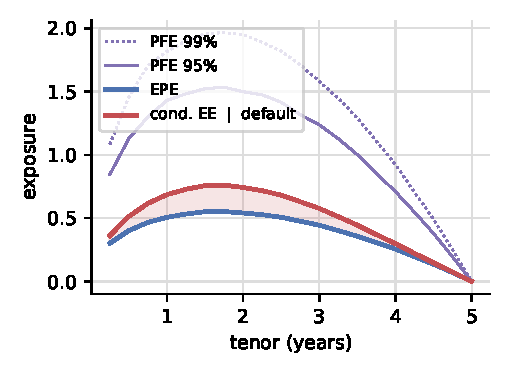
\includegraphics[width=0.72\textwidth]{figs/exposure.pdf}
\caption{Exposure profiles for the five-year swap. The shaded band is the
wrong-way adjustment: the conditional EE given default (Hull--White, $b=0.6$)
dominates the independent EPE at every tenor.}
\label{fig:exposure}
\end{figure}

\begin{figure}[t]
\centering
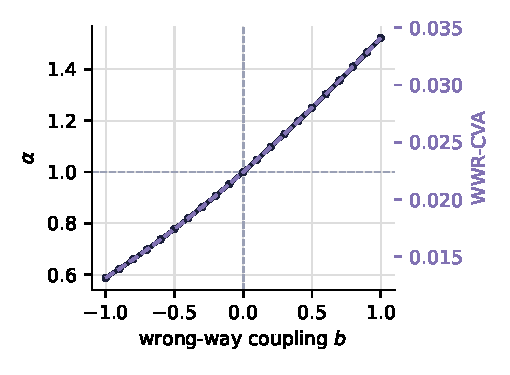
\includegraphics[width=0.72\textwidth]{figs/alpha_sweep.pdf}
\caption{Multiplier $\alpha$ (left axis) and $\CVA_{\text{WWR}}$ (right axis)
versus the coupling $b$. Both are monotone in $b$ and cross $\alpha=1$ at $b=0$,
as proved in Theorem~\ref{thm:mono}.}
\label{fig:sweep}
\end{figure}

At $b=0.6$ the independent CVA $0.02240$ rises to $0.02918$, a $+30.3\%$ uplift,
$\alpha=1.30$, with $\EEPE=0.524$ and $\EAD=0.683$ (normalised units).
Table~\ref{tab:models} compares dependence families at illustrative strengths;
the tail-dependent Clayton copula produces the largest uplift, consistent with
defaults concentrating in the exposure tail.

\begin{table}[t]
\centering
\caption{Wrong-way risk multiplier across dependence models (five-year swap).}
\label{tab:models}
\begin{tabular}{lcc}
\toprule
Model & $\alpha$ & Uplift \\
\midrule
Hull--White ($b=0.6$)    & 1.30 & $+30.3\%$ \\
Gaussian ($\rho=0.5$)    & 2.54 & $+153.8\%$ \\
Frank ($\theta=5$)       & 2.12 & $+111.9\%$ \\
Clayton ($\theta=2$)     & 4.11 & $+311.0\%$ \\
\bottomrule
\end{tabular}
\end{table}

Figure~\ref{fig:marg} verifies Proposition~\ref{prop:marg} numerically: the
model-implied marginal PDs coincide with the curve targets to a maximum absolute
error of $8.5\times10^{-16}$, i.e.\ machine precision.

\begin{figure}[t]
\centering
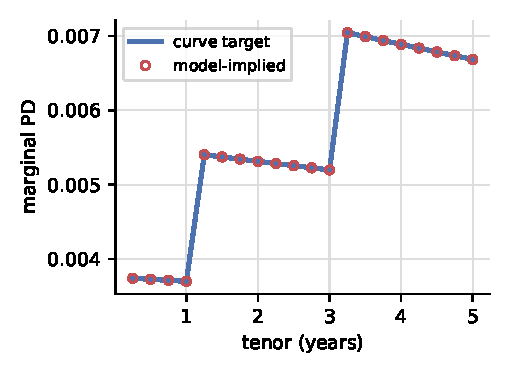
\includegraphics[width=0.72\textwidth]{figs/marginal.pdf}
\caption{Arbitrage consistency: the Hull--White model-implied marginal PDs sit
exactly on the curve targets (maximum error $8.5\times10^{-16}$).}
\label{fig:marg}
\end{figure}

\section{Reproducibility and symbolic verification}\label{sec:verif}
Every stochastic operation accepts an explicit seed, so results are bit-for-bit
reproducible. Beyond numerical acceptance tests, the structural identities of
Sections~\ref{sec:model}--\ref{sec:inverse} are \emph{machine-checked} with the
SymPy computer-algebra system: equations~\eqref{eq:clayton}--\eqref{eq:frank}
are confirmed to equal $\partial_v C$ for the Clayton and Frank copulas; the
survival/PD telescoping, the piecewise cumulative-hazard integral,
Proposition~\ref{prop:marg}, the softmax normalisation, the Gaussian threshold
of~\eqref{eq:gauss}, the CVA integrand~\eqref{eq:cva}, and the score identity of
Lemma~\ref{lem:cov} are each reduced symbolically to zero. The core attains
$100\%$ line coverage; the static type checker and linter pass cleanly. The
library is released under the MIT licence with documentation, an interactive
browser playground, and the figures of this paper fully reproducible from
source.

\section{Conclusion}
\emph{wayfault} packages a complete, auditable WWR workflow behind a numpy-only
core. The unifying re-weighting view places stochastic-hazard and copula models
on a common footing, and the proven monotonicity of $\alpha$ underwrites a novel
\emph{prescriptive} layer: calibrating dependence to a target multiplier or CVA,
and locating reverse-stress breakpoints. Natural extensions include bootstrap
confidence intervals for $\alpha$ and a model-free, information-theoretic WWR
intensity.

\begin{thebibliography}{9}
\bibitem[Hull and White(2012)]{hullwhite2012}
J.~Hull and A.~White. CVA and wrong-way risk.
\emph{Financial Analysts Journal}, 68(5):58--69, 2012.
\bibitem[Gregory(2015)]{gregory}
J.~Gregory. \emph{The xVA Challenge: Counterparty Risk, Funding, Collateral,
and Capital}. Wiley, 3rd edition, 2015.
\bibitem[BCBS(2011)]{basel}
Basel Committee on Banking Supervision. Basel III: A global regulatory framework
for more resilient banks and banking systems. BIS, 2011.
\bibitem[Nelsen(2006)]{nelsen}
R.~B. Nelsen. \emph{An Introduction to Copulas}. Springer, 2nd edition, 2006.
\end{thebibliography}

\end{document}
